% Limit order book depth diagram.
% Horizontal bars: each price level is one row, bar length = quantity.
% Asks (sellers) above in red, bids (buyers) below in blue. The spread
% is the gap between best bid (100) and best ask (101).

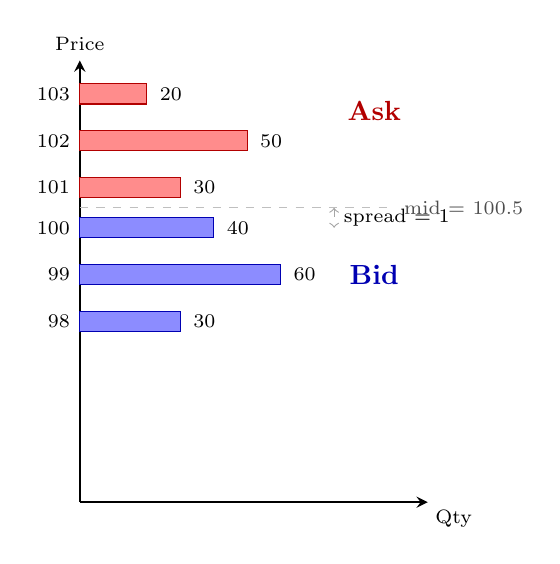
\begin{tikzpicture}[
    scale=0.85,
    every node/.style={font=\scriptsize},
    bidbar/.style={fill=blue!45, draw=blue!70!black},
    askbar/.style={fill=red!45,  draw=red!70!black},
]

% Axes
\draw[->, thick, >=stealth] (0,0) -- (5.2,0) node[below right=-1pt] {Qty};
\draw[->, thick, >=stealth] (0,0) -- (0,6.6) node[above] {Price};

% Asks (descending from best ask at 101, drawn above the mid line)
%   y-position chosen so each level sits on its own row
\node[left] at (0, 6.10) {103};
\filldraw[askbar] (0, 5.95) rectangle (1.0, 6.25);
\node[right] at (1.05, 6.10) {20};

\node[left] at (0, 5.40) {102};
\filldraw[askbar] (0, 5.25) rectangle (2.5, 5.55);
\node[right] at (2.55, 5.40) {50};

\node[left] at (0, 4.70) {101};
\filldraw[askbar] (0, 4.55) rectangle (1.5, 4.85);
\node[right] at (1.55, 4.70) {30};

% Spread annotation between best ask (101) and best bid (100)
\draw[<->, dashed, gray!70] (3.8, 4.40) -- (3.8, 4.10);
\node[right] at (3.8, 4.25) {spread = 1};

% Bids (descending from best bid at 100, drawn below the mid line)
\node[left] at (0, 4.10) {100};
\filldraw[bidbar] (0, 3.95) rectangle (2.0, 4.25);
\node[right] at (2.05, 4.10) {40};

\node[left] at (0, 3.40) {99};
\filldraw[bidbar] (0, 3.25) rectangle (3.0, 3.55);
\node[right] at (3.05, 3.40) {60};

\node[left] at (0, 2.70) {98};
\filldraw[bidbar] (0, 2.55) rectangle (1.5, 2.85);
\node[right] at (1.55, 2.70) {30};

% Mid price dashed line
\draw[dashed, gray!50] (0, 4.40) -- (4.7, 4.40);
\node[right, gray!60!black] at (4.7, 4.40) {mid = 100.5};

% Side labels
\node[red!70!black,  font=\bfseries] at (4.4, 5.85) {Ask};
\node[blue!70!black, font=\bfseries] at (4.4, 3.40) {Bid};

\end{tikzpicture}